\documentclass{llncs}
\usepackage{makeidx}  % allows for indexgeneration
\usepackage{hyperref}
\usepackage{graphicx}
\usepackage{todonotes}

\begin{document}

\title{Testing OWL Axioms Against RDF Facts:\\
A possibilistic approach based on falsifiability}
%
\titlerunning{Testing OWL Axioms}  % abbreviated title (for running head)
%                                     also used for the TOC unless
%                                     \toctitle is used
%
\author{Andrea G. B. Tettamanzi\inst{1} \and Catherine Faron-Zucker\inst{1} \and Fabien Gandon\inst{2}}
%
\authorrunning{Andrea G. B. Tettamanzi et al.} % abbreviated author list (for running head)
%
%%%% list of authors for the TOC (use if author list has to be modified)
%\tocauthor{Ivar Ekeland, Roger Temam, Jeffrey Dean, David Grove,
%Craig Chambers, Kim B. Bruce, and Elisa Bertino}
%
\institute{Universit\'e Nice Sophia Antipolis, I3S, UMR 7271, Sophia Antipolis, France,\\
\email{andrea.tettamanzi@unice.fr}, \email{faron@polytech.unice.fr}
\and
INRIA, Sophia Antipolis, France,\\
\email{fabien.gandon@inria.fr}}

% Submission 176

\maketitle

\begin{abstract} %Min 70, max 150 words:
Automatic knowledge base enrichment methods rely critically on candidate axiom scoring.
The most popular scoring heuristics proposed in the literature are based on statistical inference.
We argue that such a probability-based framework is not always completely satisfactory.
To solve its issues, we propose to approach the problem from an epistemological perspective.
In particular, we argue that Karl Popper's critical rationalism provides a suitable
foundation for axiom induction. Based on it, we propose a novel, alternative scoring
heuristics expressed in terms of possibility theory, whereby a candidate axiom receives
a bipolar score consisting of a degree of possibility and a degree of necessity.
We evaluate our proposal by applying it to the problem of testing \textsf{SubClassOf}
axioms against the DBpedia RDF dataset.

% Mots clés à ajouter/enlever ?
\keywords{ontology learning, open-world assumption, falsification, possibility theory}
\end{abstract}

\section{Introduction}

The common approach to the semantic Web puts strong emphasis
on a principled conceptual analysis of a domain of interest
leading to the construction or reuse of ontologies
as a prerequisite step for the organization of the Linked Open Data (LOD),
much like a database schema must be designed before a database can be populated,
in the wake of a time-honored tradition of knowledge engineering in artificial intelligence.

This approach has some limitations:
it is aprioristic and dogmatic in the way knowledge should be organized;
while it is quite successful when applied to specific domains,
it does not scale well to more general settings;
it does not lend itself to a collaborative effort; etc.

That is why an alternative, bottom-up, \emph{grass-roots} approach to ontology and
knowledge base creation is beginning to emerge: instead of postulating an \emph{a priori}
conceptualization of reality (i.e., an ontology) and requiring that our knowledge
about facts complies with it, one can start from raw data and learn their schema
or start from RDF facts and learn OWL~2 axioms.

Recent contributions towards the automatic creation of OWL~2 ontologies
from large repositories of RDF facts include
FOIL-like algorithms for learning concept definitions~\cite{FanizziDAmatoEsposito2008},
statistical schema induction via association rule mining~\cite{FleischhackerVoelkerStuckenschmidt2012},
and light-weight schema enrichment methods based on the DL-Learner
framework~\cite{HellmannLehmannAuer2009,BuehmannLehmann2012}.
All these methods apply and extend techniques developed within inductive logic programming
(ILP)~\cite{ILPat20}.

On a related note, there exists a need for evaluating and validating ontologies,
be they the result of an analysis effort or of a semi-automatic learning method.
This need is witnessed by general methodological investigations
\cite{GangemiCatenacciCiaramitaLehmann2005,GangemiCatenacciCiaramitaLehmann2006}
and surveys \cite{TartirBudakArpinarSheth2007} and tools like OOPS! \cite{PovedaSuarezGomez2012}
for detecting pitfalls in ontologies.

Checking whether a given OWL~2 ontology does make sense and correctly reflect reality
is like testing a computer program for correctness, in a sense, or a scientific hypothesis.
Ontology engineering methodologies, such as METHONTOLOGY~\cite{FernandezGomezJuristo1997},
distinguish two validation activities, namely verification (through formal methods, syntax, logics, etc.)
and validation through usage. Whilst this latter is usually thought of as user studies,
an automatic process of validation based on RDF data would provide a cheap alternative,
whereby the existing linked data may be regarded as usage traces that can be used
to test and improve the ontologies, much like log mining can be used to provide
test cases for development in the replay approaches.
%Conceptually, this amounts to adding all the known facts to the ontology as
%assertion axioms and checking whether consistency is preserved;
%things, however, are complicated by the fact that large RDF repositories resulting from
%the automatic extraction of data from collaborative efforts, like DBpedia,\footnote{\url{http://dbpedia.org}}
%tend to be noisy and incomplete. 
Alternatively, one may regard the ontology as a set of integrity constraints and check if the
data satisfy them, using a tool like Pellet integrity constraint validator (ICV),
which translates OWL integrity constraint ontologies into SPARQL queries automatically
to validate RDF data~\cite{SirinTao2009}.
A similar approach also underlies the idea of test-driven evaluation of linked data 
quality~\cite{KontokostasWestphalAuerHellmannLehmannCornelissen2014}.
To this end, OWL ontologies are interpreted under the closed-world assumption and
the weak unique name assumption. 

Yet this validation process may be seen from a reverse point of view:
instead of starting from the \emph{a priori} assumption that a given ontology
is correct and verify whether the facts contained in an RDF base satisfy it,
one may treat ontologies like hypotheses and develop a methodology to verify
whether the RDF facts corroborate or falsify them. Ontology learning and validation
are thus strictly related.
They could even be seen as an agile and test-driven approach to ontology development,
where the linked data is used as a giant test case library not only to validate the
schema but even to suggest new developments.

Ontology learning and validation rely critically on (candidate) axiom scoring.
The most popular scoring heuristics proposed in the literature are based on statistical inference.
We argue that such a probability-based framework is not always completely satisfactory.

In this paper, we will tackle the problem of testing a single, isolated axiom,
which is anyway the first step to solve the problem of validating an entire ontology.
Furthermore, to keep things reasonably simple, we will restrict our attention
to subsumption axioms of the form $\mathsf{SubClassOf}(C\ D)$.
We will propose an evaluation of the degree of corroboration of axioms
based on possibility theory, using such a setting to formalize some key ideas
from Karl Popper's approach to epistemology, like the notions of logical content
of a theory and of falsification. Our research question is: ``can we apply the
falsifiability criterion, which lays at the foundations of the scientific method,
to the task of testing candidate axioms for ontology learning?''.
In addition, ``could this be beneficial to ontology and knowledge base validation?''

The paper is organized as follows:
Section~\ref{probability} reviews probability-based scoring heuristics and
points out some of their issues; Section~\ref{epistemology} approaches the
problem of axiom induction from an epistemological perspective and
Section~\ref{possibility-theory} proposes an alternative heuristics based
on possibility theory. The implementation of the heuristics is then detailed in
Section~\ref{OWL2SPARQL} and an evaluation is provided in Section~\ref{evaluation}.
Section~\ref{conclusion} concludes.

\section{Probability-Based Candidate Axiom Scoring}
\label{probability}

A statistics-based heuristics for the scoring of candidate axioms used
in the framework of knowledge base enrichment~\cite{BuehmannLehmann2012}
may be regarded essentially as scoring an axiom by an estimate of the probability
that one of its logical consequences is confirmed (or, alternatively, falsified)
by the facts stored in the RDF repository.

This relies on the assumption of a binomial distribution, which applies when an
experiment (here, checking if a logical consequence of a candidate axiom is confirmed
by the facts) is repeated a fixed number of times, each trial having two possible outcomes
(conventionally labeled \emph{success} and \emph{failure}; here, we might call them
\emph{confirmation}, if the observed fact agrees with the candidate axiom,
and \emph{counterexample}, if the observed fact contradicts it),
the probability of success being the same for each trial,
and the trials being statistically independent.

We will use the following notation throughout the paper:
let $\phi$ be a candidate axiom; we will denote by $u_\phi$ the support or sample size for $\phi$,
i.e., the cardinality of the set of its logical consequences that will be tested in the RDF repository,
by $u_\phi^+$ the number of such consequences which are true (confirmations), and
by $u_\phi^-$ the number of such consequences which are false (counterexamples).
%Notice that $u_\phi^+$ will be at most the cardinality of the truth content of $\phi$,
%while $u_\phi^-$ will be at most the cardinality of the falsity content of $\phi$.
A few interesting properties of these three cardinalities are:
\begin{eqnarray}
  u_\phi^+ + u_\phi^- &\leq& u_\phi;\label{eq:conf-pls-expt-lt-refc} \\
  u_\phi^+ &=& u_{\neg\phi}^-; \\
  u_\phi^- &=& u_{\neg\phi}^+; \\
  u_\phi &=& u_{\neg\phi}.
\end{eqnarray}


As B\"uhmann and Lehmann point out~\cite{BuehmannLehmann2012},
estimating the probability of confirmation of axiom $\phi$ just by $\hat{p}_\phi = u_\phi^+/u_\phi$
would be too crude and would not take the magnitude of $u_\phi$ into account.
The parameter estimation must be carried out by performing a statistical inference.

One of the most basic analyses in statistical inference is to form a confidence interval
for a binomial parameter $p_\phi$ (probability of confirmation of axiom $\phi$), given
a binomial variate $u_\phi^+$ for sample size $u_\phi$ and a sample proportion $\hat{p}_\phi = u_\phi^+/u_\phi$.
Most introductory statistics textbooks use to this end the Wald confidence interval,
based on the asymptotic normality of $\hat{p}_\phi$ and estimating the standard error.
This $(1 - \alpha)$ confidence interval for $p_\phi$ would be
\begin{equation}\label{eq:Wald}
  \hat{p}_\phi \pm z_{\alpha/2}\sqrt{\hat{p}_\phi(1 - \hat{p}_\phi)/u_\phi},
\end{equation}
where $z_c$ denotes the $1 - c$ quantile of the standard normal distribution.

However, the central limit theorem applies poorly to this binomial distribution
with $u_\phi<30$ or where $\hat{p}_\phi$ is close to 0 or 1.
The normal approximation fails totally when $\hat{p}_\phi = 0$ or $\hat{p}_\phi = 1$.
That is why B\"uhmann and Lehmann~\cite{BuehmannLehmann2012} base their probabilistic score
on Agresti and Coull's binomial proportion confidence interval~\cite{AgrestiCoull1998},
an adjustment of the Wald confidence interval which goes: ``Add two successes and two failures
and then use Formula~\ref{eq:Wald}.'' Such adjustment is specific for constructing
95\% confidence intervals.

%In fact, Agresti and Coull's suggestion is a simplification of the Wilson score interval,
%%\begin{equation}
%%  \left(
%%    \hat{p}_\phi + \frac{z_{\alpha/2}^2}{2u_\phi} \pm
%%    z_{\alpha/2}\sqrt{\frac{\hat{p}_\phi(1 - \hat{p}_\phi) + \frac{z_{\alpha/2}^2}{4u_\phi}}{u_\phi}}
%%  \right) / \left(1 + \frac{z_{\alpha/2}^2}{2u_\phi}\right),
%%\end{equation}
%which is an approximate binomial confidence interval obtained by inverting the approximately
%normal test that uses the null, rather than the estimated, standard error.
%When used to compute the 95\% score interval, this confidence interval
%has coverage probabilities close to the nominal confidence level and can be recommended
%for use with nearly all sample sizes and parameter values.

A remark about such approaches is in order. They only look for confirmations of $\phi$, and treat
the absence of a confirmation as a failure in the calculation of the confidence interval.
This is like making an implicit closed-world assumption. In reality, definitions
of explicit failures, or \emph{counterexamples}, can be given (see, e.g.,
the one we will propose in Section~\ref{OWL2SPARQL}), but then the probability
of finding a confirmation and the probability of finding a counterexample do not necessarily add to one,
because there is a non-zero probability of finding neither a confirmation nor a counterexample
for every potential falsifier of an axiom, as stated in Equation~\ref{eq:conf-pls-expt-lt-refc}.
For example, in DBpedia dataset, axiom
\textsf{SubClassOf}(\textsf{dbo:LaunchPad} \textsf{dbo:Infrastructure}) has 85 potential
falsifiers, 83 confirmations and 1 counterexample; the probability of finding neither a
confirmation nor a counterexample for any potential falsifier is thus 1.1765\%.
B\"uhmann and Lehmann's scoring method should thus be
corrected in view of the open-world assumption, for example by using
$\hat{p}^* = u_\phi^+/(u_\phi^+ + u_\phi^-)$ as the sample proportion instead of $\hat{p}$.

However, there is a more fundamental critique to the very idea of computing the likelihood
of axioms based on probabilities. In essence, this idea relies on the assumption
that it is possible to compute the probability that an axiom $\phi$ is true given
some evidence $e$, for example $e$ = ``$\psi$ such that $\phi\models\psi$ is in the RDF repository'',
or $e$ = ``$\psi$ such that $\psi\models\neg\phi$ is in the RDF repository'',
or $e$ = ``$\psi$ such that $\phi\models\psi$ is \emph{not} in the RDF repository'', etc.,
which, by Bayes' formula, may be written as
\begin{equation}
  \Pr(\phi \mid e) = \frac{\Pr(e \mid \phi)\Pr(e)}{\Pr(e \mid \phi)\Pr(e) + \Pr(e \mid \neg\phi)\Pr(\neg e)}.
\end{equation}
Therefore, in order to compute (or estimate) such probability,
one should at least be able to estimate probabilities such as
\begin{itemize}
\item the probability that a fact confirming $\phi$ is added to the repository
  given that $\phi$ holds;
\item the probability that a fact contradicting $\phi$ is added to the repository
  in error, i.e., given that $\phi$ holds;
\item the probability that a fact confirming $\phi$ is added to the repository
  in error, i.e., given that $\phi$ does not hold;
\item the probability that a fact contradicting $\phi$ is added to the repository
  given that $\phi$ does not hold.
\end{itemize}
Now, it is not hard to argue that the above probabilities may vary as a function of the
concepts and properties involved. Let us take a subsumption axiom $\mathsf{SubClassOf}(C\ D)$
as an example. A fact confirming it is $D(a)$, with $C(a)$ in the dataset,
whereas a fact contradicting it is $E(a)$, with $C(a)$ in the dataset
and $\mathsf{DisjointClasses}(E\ D)$ in the ontology.
Assuming that $\mathsf{SubClassOf}(C\ D)$ holds, we may suspect that
$D(a)$ is more likely to be found in the repository
if $D$ is either very specific (and thus ``closer'' to $a$ or very general (like
\textsf{foaf:Person}), and less likely if it is somewhere in the middle.
This supposition is based on our expectations of what people are likely to say
about $a$. For instance, an average person, if asked ``what is this?'' when pointing
to a basset hound, is more likely to answer ``a dog'' or ``an animal'' than,
say, ``a carnivore'' or ``a mammal'', which, on purely logical grounds,
would be perfectly valid things to say about it~\cite{Lakoff1987}.
% a phenomenon which John Sowa called \emph{salience} of an ontological or linguistic term.
There is thus an inherent difficulty with estimating the above probabilities,
one which cannot be solved otherwise than by performing a large number of
experiments, whose results, then, would be hard to generalize.
By this argument, any axiom scoring method based on probability or statistics is doomed
to be largely arbitrary and potentially fallacious.


\section{Induction from an Epistemological Perspective}
\label{epistemology}

The difficulties highlighted in the previous section suggest that a more
principled approach is needed. To solve them, we should turn to epistemology,
the branch of philosophy that studies how knowledge is acquired.
Discovering axioms from a finite, albeit huge, set of known facts
may be regarded as a form of inductive reasoning, in that it proceeds
from particular instances of concepts and relations (RDF triples)
to broader generalizations (axioms).

The \emph{problem of induction} is the question whether, or under which conditions,
and to what degree, inductive inferences are justified.
Karl Popper is the one philosopher that made the most valuable contribution
to our understanding of the problem of induction, by proposing the principle
of \emph{falsifiability} \cite{Popper1935}, which lies at the foundation of his critical rationalism:
all knowledge is provisional, conjectural, hypothetical---we can never finally
prove our scientific theories, we can merely (provisionally) confirm or
(conclusively) refute them.

We may define the statement that an observation refutes, or contradicts, a hypothesis
as equivalent to the statement that an ontology containing the axiom corresponding to the hypothesis
and the dataset containing the assertion corresponding to the observation together make an
inconsistent knowledge base.

While the definition of ``contradict'' is clear enough not to be subject to debate,
defining what it means to ``confirm'' a hypothesis is much trickier. This is
of course closely related to Popper's observation that a hypothesis can never be
conclusively confirmed.

The difficulty of finding a satisfactory and intuitive definition of confirmation
is witnessed by Hempel's paradox~\cite{Hempel1945}:
if we suppose (i) that a simple universal condition (``all ravens are black'')
is satisfied by the joint satisfaction of its antecedent and consequent, and we
also accept (ii) that whatever confirms a statement confirms also all its logical
equivalents (e.g., ``all non-black things are not ravens'') --- the \emph{equivalence hypothesis},
then we must conclude that a blue chair, for example, confirms the hypothesis
that all ravens are black, even though it has nothing to do with ravens! 

Although Hempel's solution of this paradox was to accept the paradoxical conclusion
and argue that our intuition is biased by our background knowledge, the most popular
solution is to approach it from a statistical point of view. The key of this solution
is to assign a weight to evidence in terms of the Bayes factor. 
The hypothesis ``all ravens are black'' may be
written $\mathsf{Raven} \sqsubseteq \mathsf{Black}$ in a description logic language and the equivalence hypothesis $\neg\mathsf{Black} \sqsubseteq \neg\mathsf{Raven}$.
Then deciding whether
$\mathsf{Raven} \sqsubseteq \mathsf{Black}$ is true, rather than its contrary, on the basis
of some observed data $D$ may be stated as a model selection problem in which the two
``models'' may be assessed by the Bayes factor
\begin{equation}
  K = \frac{\Pr(D \mid \mathsf{Raven} \sqsubseteq \mathsf{Black})}{\Pr(D \mid \mathsf{Raven} \not\sqsubseteq \mathsf{Black})}.
\end{equation}
Then, observing a green apple does indeed confirm our hypothesis, but its weight
is much lower than observing a black raven, just because there are so many more non-ravens in the
Universe than ravens and so many colors those objects can be of. This argument, which
is known as the Bayesian solution to Hempel's paradox, seems convincing enough,
but it cannot be blindly accepted in all contexts.

In fact, the key argument for rejecting a probabilistic approach in the specific context of axiom induction from an RDF dataset like DBpedia is to observe that it contains facts automatically extracted from Wikipedia,
which is the result of a collaborative effort, whose coverage is not planned and
subject to cultural and historical biases.\footnote{For example, at the level
of pop music, the coverage of DBpedia is very much biased towards anglophone artists.
Even in domains, such as geographical data, which one would expect to be much more
uniform and extensive, it turns out that the coverage of Wikipedia is far from being uniform.}
%cath see, e.g., Denny Vrandecic's post on a map of all Wikipedia articles, \url{https://plus.google.com/+DennyVrandecic/posts/XmMWKuzJvpV} 
%cath je ne trouve pas d'article à citer

Therefore, there is no reason to assume that the facts contained in an RDF triple store
be \emph{representative} of all possible facts that could be recorded, unless
that RDF store is the result of a planned and well-designed effort aimed at building
a knowledge base providing uniform coverage of a given domain.
Indeed, to use the number of facts supporting a hypothesis
to estimate its probability one would have to make the very strong assumption
that the finite set of facts in the RDF store is a representative sample
of the infinite set of all ``real'' facts, whatever this means.
Adopting a probabilistic approach whereas its assumptions are not
fulfilled might lead to fallacious results.

Applying Popper's idea of falsifiability to the induction problem,
Scheffler and Goodman introduced the concept of \emph{selective confirmation}
\cite{SchefflerGoodman1972}, whereby evidence may be characterized
not simply as satisfying a hypothesis, but, further, as favoring the hypothesis
rather than its contrary.
Thus, evidence of a black raven \emph{selectively confirms} the hypothesis
$\mathsf{Raven} \sqsubseteq \mathsf{Black}$ because it both confirms it and fails to confirm its
negation, $\mathsf{Raven} \not\sqsubseteq \mathsf{Black}$, namely
that there exist ravens that are not black. On the contrary, the observation of
a green apple does not contradict $\mathsf{Raven} \sqsubseteq \mathsf{Black}$,
but it does not disconfirm $\mathsf{Raven} \not\sqsubseteq \mathsf{Black}$
either; therefore, it does not selectively confirm $\mathsf{Raven} \sqsubseteq \mathsf{Black}$.
Selective confirmation is a nice example of a definition of ``providing evidence in favor of'',
which does not coincide with or imply ``increasing the probability of''.
We will adopt such a definition.


\section{A Possibilistic Candidate Axiom Scoring Heuristic}
\label{possibility-theory}

We propose here two functions for evaluating the possibility and the necessity of
an axiom which try to model the basic intuition behind this induction process
in light of the discussion provided in Section~\ref{epistemology}.
To define these notions we rely on possibility theory.


\subsection{Possibility Theory}
\label{PossibilityTheory}

Possibility theory \cite{Zadeh1978} is a mathematical theory of epistemic uncertainty.
Given a finite universe of discourse $\Omega$, whose elements $\omega\in\Omega$
may be regarded as events, values of a variable, possible worlds, or states of affairs,
a possibility distribution is a mapping $\pi: \Omega \to [0, 1]$,
which assigns to each $\omega$ a degree of possibility ranging from 0 (impossible,
excluded) to 1 (completely possible, normal).
A possibility distribution for  which there exists a completely possible state of
affairs ($\exists \omega^*: \pi(\omega^*) = 1$) is said to be \emph{normalized}.

There is a similarity between possibility distribution and probability 
density. However, it must be stressed that $\pi(\omega) = 1$ just means that
$\omega$ is a plausible (normal) situation and therefore should not be excluded.
A degree of possibility can then be viewed as an upper bound of a degree of probability.
Possibility theory is suitable to represent incomplete knowledge while 
probability is adapted to represent random and observed phenomena. 
We invite the reader to see~\cite{dubois1991} for more informations
about the relationships between fuzzy sets, possibility, and probability 
degrees.

A possibility distribution $\pi$ induces a \emph{possibility
measure}\index{possibility measure} and its dual \emph{necessity
measure}\index{necessity measure}, denoted by $\Pi$ and $N$
respectively. Both measures apply to a set $A \subseteq\Omega$ (or to a
formula $\phi$, by way of the set of its models, $A = \{\omega : \omega \models \phi\}$),
and are defined as follows:
\begin{eqnarray}
  \Pi(A) &=& \max_{\omega\in A} \pi(\omega); \\
  N(A)   &=& 1 - \Pi(\bar{A}) = \min_{\omega\in \bar{A}} \{1 - \pi(\omega)\}.
\end{eqnarray}

In words, the possibility measure of $A$ corresponds to the
greatest of the possibilities associated to its elements; conversely,
the necessity measure of $A$ is equivalent to the impossibility of
its complement $\bar{A}$.

A few properties of possibility and necessity measures 
induced by a normalized possibility distribution on a finite universe of
discourse $\Omega$ are the following. For all subsets $A, B\subseteq \Omega$:
\begin{enumerate}
  \item $\Pi(A \cup B) = \max\{\Pi(A), \Pi(B)\}$;
  \item $\Pi(A \cup \bar A) = \max\{\Pi(A), \Pi(\bar A)\}=1$;
  \item $\Pi(\emptyset) = N(\emptyset) = 0$,\quad $\Pi(\Omega) = N(\Omega) = 1$;
  \item $N(A \cap B) = \min\{N(A), N(B)\}$;
  \item $\Pi(A) = 1 - N(\bar{A})$ (duality);
  \item $N(A) \leq \Pi(A)$;
  \item $N(A) > 0$ implies $\Pi(A) = 1$;
  \item $\Pi(A) < 1$ implies $N(A) = 0$.
\end{enumerate}
In case of complete ignorance on $A$, $\Pi(A) = \Pi(\bar{A}) = 1$.

\subsection{The Case for a Possibilistic Approach}

Popper introduces the concept of \emph{degree of corroboration}, which makes us think
of an attempt at something like possibility theory, which, it should be noted, was
yet to come at the time Popper developed his ideas.
A confirmation that what Popper calls degree of corroboration of a hypothesis
is to be regarded as a possibility measure in what Popper writes on Page~19,
item~4, of \cite{Popper1972}, which may be paraphrased as follows:
given a theory $T$ and a sentence $s$ (one of its consequences),
if $T \models s$, $\mathrm{corroboration}(s) \leq \mathrm{corroboration}(T)$
and
\[
  \mathrm{corroboration}(T) = \max_{T \models s} \mathrm{corroboration}(s).
\]
It is thus tempting to draw inspiration from Popper's critical rationalism
and use the formal tools of possibility theory to devise an approach to axiom scoring. 
We can equate an axiom to a conjecture, a hypothesis in Popper's terms,
and facts contained in an RDF dataset to observations, ``basic statements''
in Popper's terms.

Popper's definition of the \emph{content} of a theory is the set of its logical consequences.
The \emph{relative content} is the set of logical consequences of the theory
given some background knowledge minus all the logical consequences of the
background knowledge (Cf.~\cite{Popper1972}, Page~49 ff.).

We formalize it as follows. 
Let $\phi$ be an axiom that we wish to evaluate (i.e., a theory). 
We define the content of $\phi$ as 
\begin{equation}\label{eq:content}
  \mathrm{content}(\phi) = \{\psi : \phi \models \psi\},
\end{equation}
\noindent
where the $\psi$ are
``basic statements'', i.e., facts that may be tested by means of a SPARQL \texttt{ASK} query.
Let $B$ be some ``background knowledge'' (a set of accepted axioms, or an existing ontology).
Then we define the content of $\phi$ relative to $B$ as
\begin{equation}\label{eq:relative-content}
  \begin{array}{rcl}
    \mathrm{content}(\phi \mid B) &=& \{\psi : B \cup \{\phi\} \models \psi \mbox{ and } B \not\models \psi\} \\
    &=& \mathrm{content}(B \cup \{\phi\}) \setminus \mathrm{content}(B).
  \end{array}
\end{equation}
Now, the \emph{truth content} of $\phi$ relative to $B$ is the subset
of $\mathrm{content}(\phi \mid B)$ which is true and the \emph{falsity content}
of $\phi$ relative to $B$ is the subset of $\mathrm{content}(\phi \mid B)$ which
is false.
For instance, $\mathrm{content}(C \sqsubseteq D)$ will include
all the facts of the form $C(x) \Rightarrow D(x)$, where $x$ may be replaced by
any individual in the dataset.

Now we can use $\mathrm{content}(\phi)$ as the set of potential falsifiers of $\phi$,
which gives
\begin{equation}\label{eq:content2}
    u_\phi = \|\mathrm{content}(\phi)\|.
\end{equation}
\noindent
% For the axiom $C \sqsubseteq D$, $u_{C \sqsubseteq D} = \|C^\mathcal{I}\|$.


\subsection{Possibility and Necessity of an Axiom}

The basic principle for establishing the possibility of a formula $\phi$ should be
that the absence of counterexamples to $\phi$ in the RDF repository means $\Pi(\phi) = 1$,
i.e., that $\phi$ is completely possible.

A hypothesis should be regarded as all the more
\emph{necessary} as it is explicitly supported by facts and not contradicted by any fact;
and all the more \emph{possible} as it is not contradicted by facts.
In other words, given hypothesis $\phi$, $\Pi(\phi) = 1$ if no counterexamples are found;
as the number of counterexamples increases, $\Pi(\phi) \to 0$ strictly monotonically;
$N(\phi) = 0$ if no confirmations are found; as the number of confirmations increases
and no counterexamples are found, $N(\phi) \to 1$ strictly monotonically.
Notice that a confirmation of $\phi$ is a counterexample of $\neg\phi$
and that a counterexample of $\phi$ is a confirmation of $\neg\phi$.

Here are a few postulates, based on our previous discussion, the possibility
and necessity functions should obey:
\begin{enumerate}
\item $\Pi(\phi) = 1$ if $u_\phi^- = 0$;
\item $N(\phi) = 0$ if $u_\phi^- > 0$ or $u_\phi^+ = 0$;
\item let $u_\phi = u_\psi$; then $\Pi(\phi) > \Pi(\psi)$ iff $u_\phi^- < u_\psi^-$;
\item let $u_\phi = u_\psi$; then $N(\phi) > N(\psi)$ iff $u_\phi^+ > u_\psi^+$ and $u_\phi^- = 0$;
\item $\lim_{u_\phi^-\to0}\frac{d\Pi(\phi)}{du_\phi^-} = -\infty$:
  the first counterexample found to an axiom should be by far the one that determines, as it were,
  the sharpest possible decrease in the degree to which we regard the axiom as possible; any further
  counterexample will only confirm our suspicions and, therefore, will provide less and less
  information;
\item $\lim_{u_\phi^+\to0}\frac{dN(\phi)}{du_\phi^+} = +\infty$:
  the first confirmation found to an axiom should be by far the one that determines, as it were,
  the sharpest possible increase in the degree to which we regard the axiom as necessary; any further
  confirmation will only add up to our acceptance and, therefore, will provide less and less
  information (cf.\ \cite{Popper1935}, \S83);
\item $\lim_{u_\phi^-\to u_\phi}\frac{d\Pi(\phi)}{du_\phi^-} = \lim_{u_\phi^+\to u_\phi}\frac{dN(\phi)}{du_\phi^+} = 0$.
\end{enumerate}

A definition of $\Pi$ and $N$ which satisfies the above postulates is, for $u_\phi > 0$,
%cath dans une version longue il faudrait le montrer
\begin{eqnarray}
  \Pi(\phi) &=& 1 - \sqrt{1 - \left(\frac{u_\phi - u_\phi^-}{u_\phi}\right)^2}; \\
  N(\phi) &=& \sqrt{1 - \left(\frac{u_\phi - u_\phi^+}{u_\phi}\right)^2}\quad
    \mbox{if $\Pi(\phi) = 1$, 0 otherwise.}
\end{eqnarray}
Notice that this is by no means the only possible definition, but we choose it because
it is the simplest one (it derives from a quadratic equation; a linear equation would
not satisfy all the postulates).
%cath dans une version longue il faudrait le montrer

%Figure~\ref{fig:poss-nec-plots} shows $\Pi(\phi)$ and $N(\phi)$ as a function of
%$u_\phi^-$ and $u_\phi^+$, respectively.
% The two functions describe an arc of an ellipse between the minor and the major axis.
It may be shown that the above definition satisfies the duality of
possibility and necessity, in that $N(\phi) = 1 - \Pi(\neg\phi)$ and
$\Pi(\phi) = 1 - N(\neg\phi)$.
As a matter of fact, we will seldom be interested in computing the necessity and
possibility degrees of the negation of OWL~2 axioms, for the simple reason that, in most cases,
the latter are not OWL~2 axioms themselves. For instance, while $C \sqsubseteq D$
is an axiom, $\neg(C \sqsubseteq D) = C \not\sqsubseteq D$ is not.


%\begin{figure}[t]
%  \begin{center}
%    \begin{tabular}{cc}
%      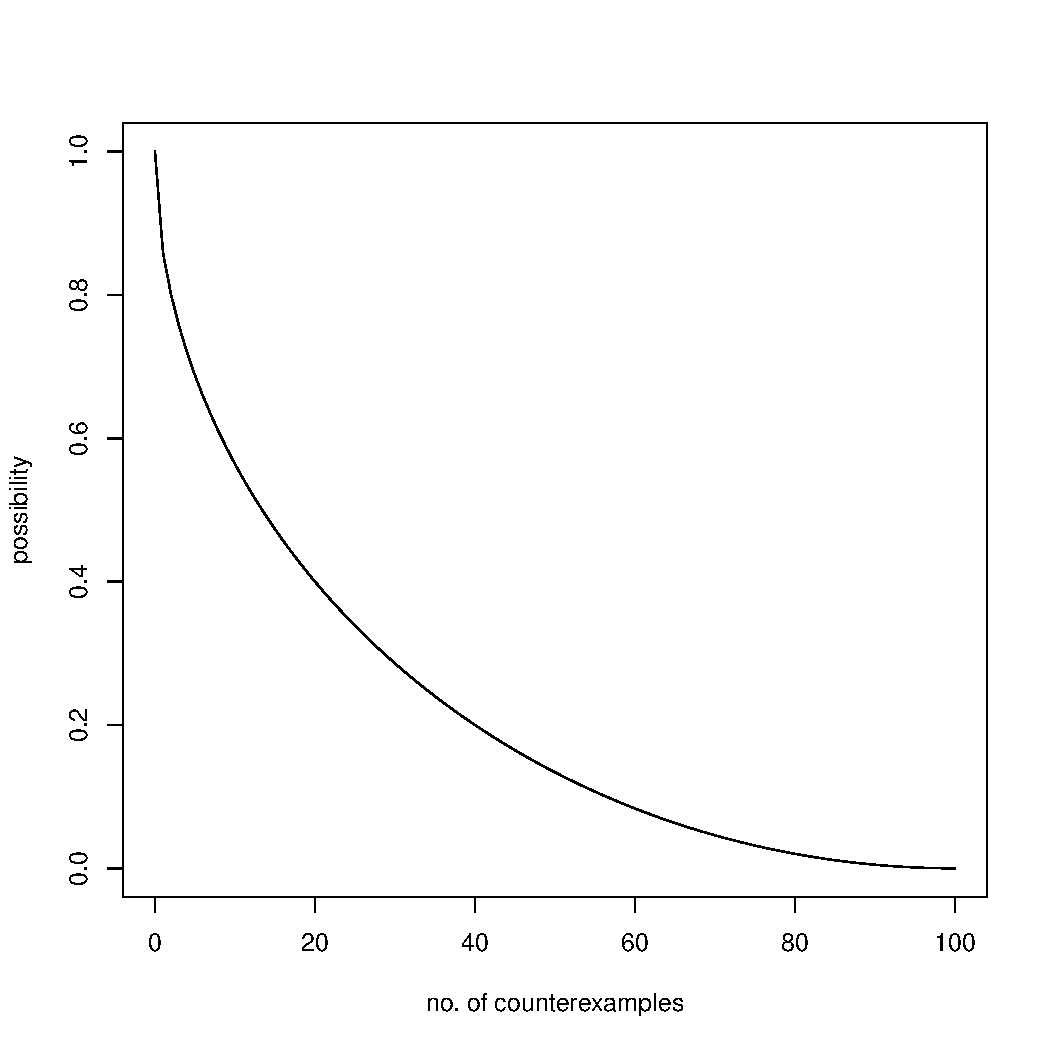
\includegraphics[width=2.25in]{../possibility} &
%      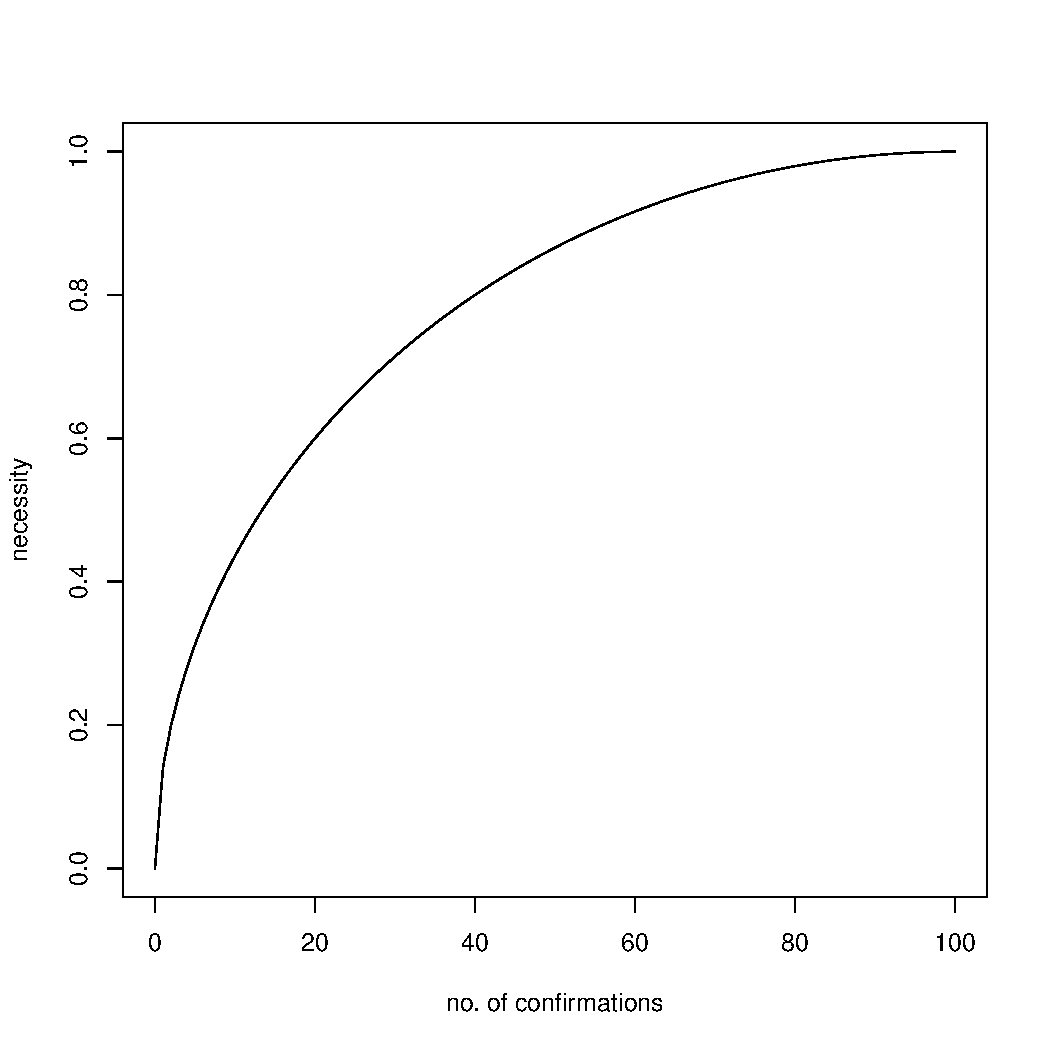
\includegraphics[width=2.25in]{../necessity} \\
%      (a) & (b)
%    \end{tabular}
%  \end{center}
%  \caption{A plot of $\Pi(\phi)$  as a function of
%    $u_\phi^-$ (a) and of $N(\phi)$ as a function of
%    $u_\phi^+$ (b) when $u_\phi = 100$.\label{fig:poss-nec-plots}}
%\end{figure}

We combine the possibility and necessity of an axiom to define
a single handy acceptance/rejection index as follows:
\begin{equation}\label{eq:ARI}
  \mathrm{ARI}(\phi) = N(\phi) - N(\neg\phi) = N(\phi) + \Pi(\phi) - 1 \in [-1, 1].
\end{equation}
A negative $\mathrm{ARI}(\phi)$ suggests rejection of $\phi$ ($\Pi(\phi)<1$),
whilst a positive $\mathrm{ARI}(\phi)$ suggests its acceptance ($N(\phi)>0$),
with a strength proportional to its absolute value. A value close to zero
reflects ignorance about the status of $\phi$.

\section{A Framework for Candidate Axiom Testing}
\label{OWL2SPARQL}

We refer to the document
\textit{OWL~2 Web Ontology Language Direct Semantics}\footnote{\url{http://www.w3.org/TR/2012/REC-owl2-direct-semantics-20121211}} for a model-theoretic semantics 
%, compatible with the description logic $\mathcal{SROIQ}$~\cite{HorrocksKutzSattler2006} 
which defines an interpretation $\mathcal{I}$ with a valuation function
$\cdot^\mathcal{I}$ mapping OWL~2 expressions into
elements and sets of elements of an interpretation domain $\Delta^\mathcal{I}$.
We take the set of all the resources that occur in a given RDF store 
as $\Delta^\mathcal{I}$ and checking an axiom 
amounts to checking whether $\mathcal{I}$ is a model of the axiom. Also, calling linked data search engines
like Sindice could virtually extend the interpretation domain to the whole LOD cloud.

However, unlike interpretation domains, RDF stores are incomplete and
possibly noisy. The open-world hypothesis must be made; therefore, absence of
supporting evidence does not necessarily contradict an axiom, and an axiom might
hold even in the face of a few counterexamples (exceptions or possible mistakes).
For example, out of 541 axioms of the form $\mathsf{SubClassOf}(C\ D)$ in the DBpedia
ontology, 143 have an empty support (i.e., class $C$ is empty)
and 28 have at least one counterexample in DBpedia 3.9.\footnote{And one, namely
\textsf{SubClassOf}(\textsf{dbo:Person} \textsf{dbo:Agent}), even has 76 counterexamples!}

%The semantics of the 32 axiom types of OWL~2 may be taken as a starting point to define,
%for each axiom type, which facts recorded in a given RDF triple store are to be taken as
%supporting evidence, or \emph{confirmations} of the axiom and which facts are to be
%construed as refuting evidence, or \emph{counterexamples}, based on the principles
%laid out in Section~\ref{epistemology}.

A general algorithm for testing all the possible OWL~2 axioms in a given RDF store is beyond the scope of this paper. 
Here, we will restrict our attention to atomic class expressions and \textsf{ObjectComplementOf}
expressions, needed to test \textsf{SubClassOf} axioms.
The model-theoretic semantics of expressions of the form $\mathsf{ObjectComplementOf}(C)$
($\neg C$ in description logics syntax), where $C$ denotes a concept expression
(called \emph{class expression} in OWL~2) is $\Delta^\mathcal{I} \setminus C^\mathcal{I}$.

Now, let us define a mapping $Q(E, x)$ from OWL~2 expressions to SPARQL graph patterns,
where $E$ is an OWL~2 expression, $x$ is a formal parameter which can take up
the name of a SPARQL variable, a resource identifier, or a literal as value,
such that the query
\texttt{SELECT DISTINCT ?x WHERE \{} $Q(E, \mbox{\tt ?x})$ \texttt{\}}
returns the extension of class expression $E$, i.e., the equivalent of $E^\mathcal{I}$,
and the query $\mbox{\tt ASK \{ } Q(E, a) \mbox{\tt\ \}}$ checks whether $E(a)$.

For an atomic concept $A$, $Q(A, \mbox{\tt ?x}) = \mbox{\tt ?x a }A\mbox{\tt .}$,
where $A$ is a valid IRI.
For concept negation, things are slightly more complicated, for RDF does not support
negation.
The obvious definition
\begin{equation}\label{eq:neg-as-failure}
  Q(\neg C, \mbox{\tt ?x}) =
    \mbox{\tt \{ ?x ?p ?o . FILTER NOT EXISTS } Q(C, \mbox{\tt ?x}) \mbox{\tt\ \}},
\end{equation}
has the problem of treating negation as failure, like in databases,
where the closed-world assumption is made. 
Since we want to preserve an open-world semantics, $Q(\neg C, x)$ should be defined
differently, as the union of the concepts that are disjoint from $C$.
One might try to express this as the set of individuals $x$ that are instances of a
concept $C'$ such that no individual $z\in C^\mathcal{I}$ is an instance of $C'$,
yielding the query
\begin{equation}\label{eq:approx-open-world-negation}
  Q(\neg C, \mbox{\tt ?x}) =
  \begin{minipage}[t]{5in}
    \begin{tabbing}
      \quad\=\quad\=\quad\=\kill
      \{\>\texttt{?x a ?dc .}\\
        \>\texttt{FILTER NOT EXISTS} \{ \texttt{?z a ?dc . } $Q(C, \mbox{\tt ?z})$ \texttt{\} \}},
    \end{tabbing}
  \end{minipage}
\end{equation}
where \texttt{?z} is a variable that does not occur anywhere else in the query.
This translation is conceptually more satisfactory than the one in Equation~\ref{eq:neg-as-failure},
but it just pushes the problem one step further, because this way of testing whether
two concepts are disjoint is based on negation as failure too.
The only way to be certain that two classes are disjoint would be to find an axiom to
this effect in the ontology:
\begin{equation}\label{eq:negation-with-disjointWith}
  Q(\neg C, \mbox{\tt ?x}) =
    \mbox{\tt \{ ?x a ?dc . ?dc owl:disjointWith }
    C \mbox{\tt\ \}},
\end{equation}
otherwise, either we find an individual which is an instance of both classes,
and thus we know the two classes are not disjoint, or we don't,
in which case the two classes may or may not be disjoint.
The fact is, very few \textsf{DisjointClasses} axioms are currently found in existing
ontologies. For example, in the DBpedia ontology, the query
\texttt{SELECT ?x ?y \{ ?x owl:disjointWith ?y \}} executed on November 22, 2013
returned 17 solutions only.
%Furthermore, we can write a query like the one in Equation~\ref{eq:negation-with-disjointWith}
%only if $C$ is an atomic concept! The definition cannot be extended to complex concepts
%because $C$ appears directly in the graph pattern, not inside a construct of the form
%$Q(C, \cdot)$, which would make induction work.
Even if not perfect, Equation~\ref{eq:approx-open-world-negation} still
represents the best available approximation to an open-world concept negation.


\section{Evaluation on Subsumption Axiom Testing}
\label{evaluation}

%All papers should include evaluations of the approaches described in the paper.
%We strongly encourage evaluations that are repeatable: preference will be given
%to papers that provide links to the data sets and queries used to evaluate their approach,
%as well as systems papers providing links to their source code or to some live deployment.

The semantics of subsumption axioms, like \textsf{SubClassOf}, may be stated in terms of set inclusion.
The model-theoretic semantics of an axiom of the form $\mathsf{SubClassOf}(C\ D)$
($C \sqsubseteq D$ in description logic syntax) is $C^\mathcal{I} \subseteq D^\mathcal{I}$.

The general principle for subsumption axioms is the following:
let us call $E_\mathrm{sub}$ and $E_\mathrm{super}$ the extensions of the subsumed and subsuming expressions, respectively, as retrieved by the relevant
SPARQL \texttt{SELECT} query. Let us then call $E_\mathrm{sub}^\neg$ and $E_\mathrm{super}^\neg$
the extension of their negated expression. Notice that, in general, this is not the
same as the complement of $E_\mathrm{sub}$ and $E_\mathrm{super}$. In fact,
$E_\mathrm{sub}^\neg \subseteq \overline{E_\mathrm{sub}}$ and
$E_\mathrm{super}^\neg \subseteq \overline{E_\mathrm{super}}$,
because of the open-world hypothesis and the fact that the RDF triple store may not
be complete. Then
\begin{itemize}
\item confirmations are those individuals $x$ such that
  $x \in E_\mathrm{sub}$ and $x \in E_\mathrm{super}$;
\item counterexamples are those individuals $x$ such that
  $x \in E_\mathrm{sub}$ and $x \in E_\mathrm{super}^\neg$.
\end{itemize}
Notice that an $x \in E_\mathrm{sub}$ such that $x \notin E_\mathrm{super}$
does not contradict a subsumption axiom, because it might well be the case
that the assertion $x \in E_\mathrm{super}$ is just missing from the ABox.
Likewise, an $x \in E_\mathrm{super}^\neg$ such that $x \in E_\mathrm{sub}^\neg$
will not be treated as a confirmation, based on our choice to regard as
evidence in favor of a hypothesis only selective confirmations.

The above general principle may be translated into specific SPARQL queries
that count the confirmations and the exceptions. For example, the two queries
to test an axiom of the form $\mathsf{SubClassOf}(C\ D)$ are
\begin{equation}
  \begin{minipage}[c]{5in}
    \begin{tabbing}
      \quad\=\quad\=\quad\=\kill
      \texttt{SELECT (count(DISTINCT ?x) AS ?numConfirmations)}\\
      \texttt{WHERE} \{ $Q(C, \mbox{\tt ?x})$ $Q(D, \mbox{\tt ?x})$ \}
    \end{tabbing}
  \end{minipage}
\end{equation}
and
\begin{equation}
  \begin{minipage}[c]{5in}
    \begin{tabbing}
      \quad\=\quad\=\quad\=\kill
      \texttt{SELECT (count(DISTINCT ?x) AS ?numExceptions)}\\
      \texttt{WHERE} \{ $Q(C, \mbox{\tt ?x})$ $Q(\neg D, \mbox{\tt ?x})$ \}
    \end{tabbing}
  \end{minipage}
\end{equation}
respectively.

We evaluated the proposed scoring heuristics by performing tests of subsumption
axioms using DBpedia 3.9 in English as the reference RDF fact repository.

In particular, on April 27, 2014, we downloaded the DBpedia dumps of English version 3.9,
generated in late March/early April 2013, along with the DBpedia ontology, version 3.9.
This local dump of DBpedia, consisting of 812,546,748 RDF triples,
has been bulk-loaded into Jena TDB and a prototype
for performing axiom tests using the proposed method has been coded in Java,
using Jena ARQ and TDB to access the RDF repository.

All experiments have been performed on a Fujitsu CELSIUS workstation equipped
with twelve six-core Intel Xeon CPU E5-2630 v2 processors at 2.60GHz clock speed,
with 15,360 KB cache each, 128 GB RAM,
4 TB of disk space with a 128 GB SSD cache,
under the Ubuntu  12.04.4 LTS 64-bit operating system.


We performed two experiments of different type: an explorative test of systematically
generated subsumption axioms and an exhaustive test of all subsumption axioms
in the DBpedia ontology.

For the former experiment, we systematically generated and tested subsumption axioms
involving atomic classes only according the following protocol:
for each of the 442 classes $C$ referred to in the RDF repository, we construct all axioms of the form
$C \sqsubseteq D$ such that $C$ and $D$ share at least one instance. Classes $D$ are obtained
with query \texttt{SELECT DISTINCT ?D WHERE \{}$Q(C, \mbox{\tt ?x})$. \texttt{?x a ?D\}}.
Due to the sheer number of axioms thus generated, and to the long time
it takes to test them,\footnote{Up to 27 hours for axiom \textsf{SubClassOf}(\textsf{dbo:Eukaryote} \textsf{dbo:Artist})!}
this experiment could not complete at the time of writing and is still underway;
however, a sufficient number of axioms was tested to allow gathering some statistics.
Figure~\ref{fig:systematic-time}a shows the distribution of test time,
while the plot of time vs.\ ARI of axioms in Figure~\ref{fig:systematic-time}b
suggests that the time it takes to test an axiom is inversely proportional to its
ARI. This is good news, because it suggests that putting a time-out
on the test would be an acceptable heuristics to decide whether to accept or reject
a candidate axiom, for an axiom which takes too long to test will likely end up
having a very negative ARI.

\begin{figure}[t]
\begin{center}
  \begin{tabular}{cc}
    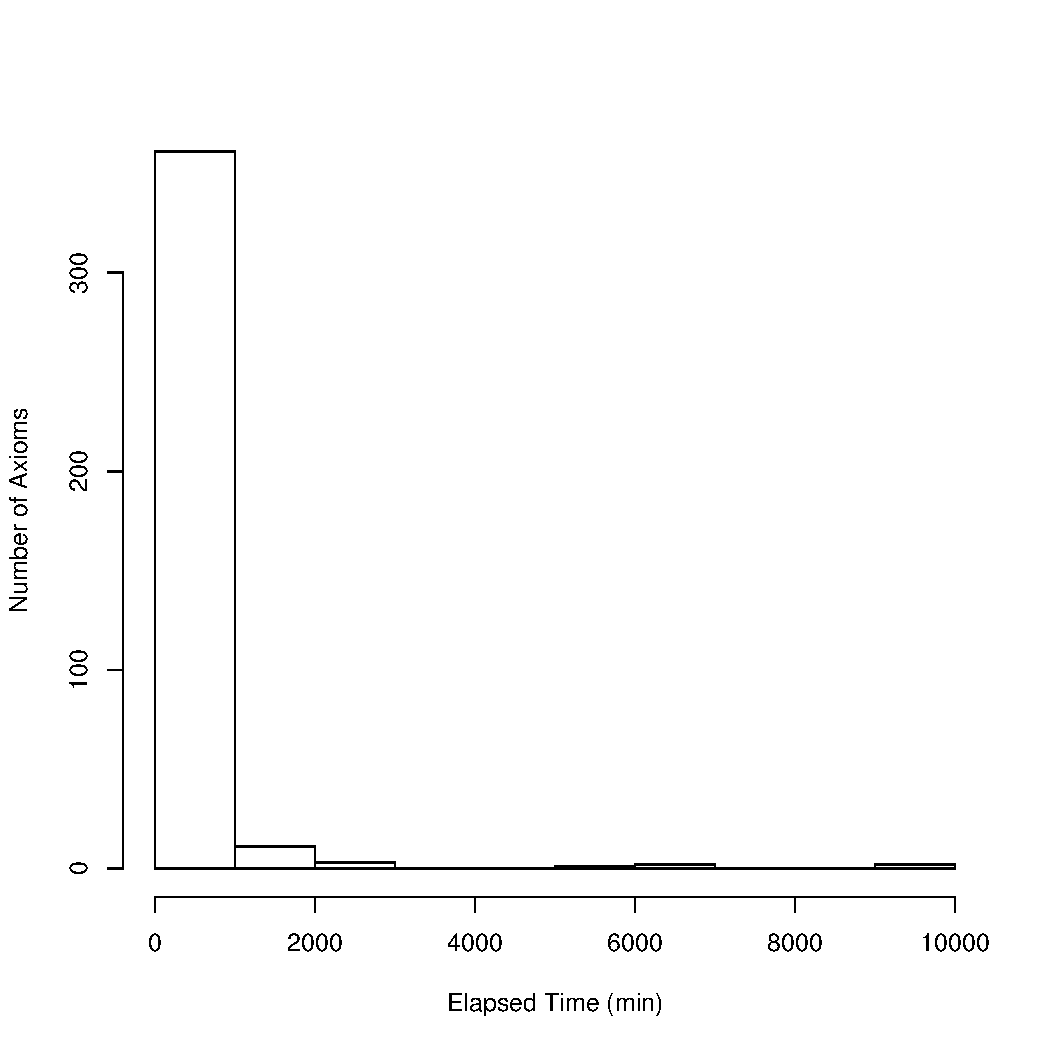
\includegraphics[height=2.25in]{systematic-time-hist} &
    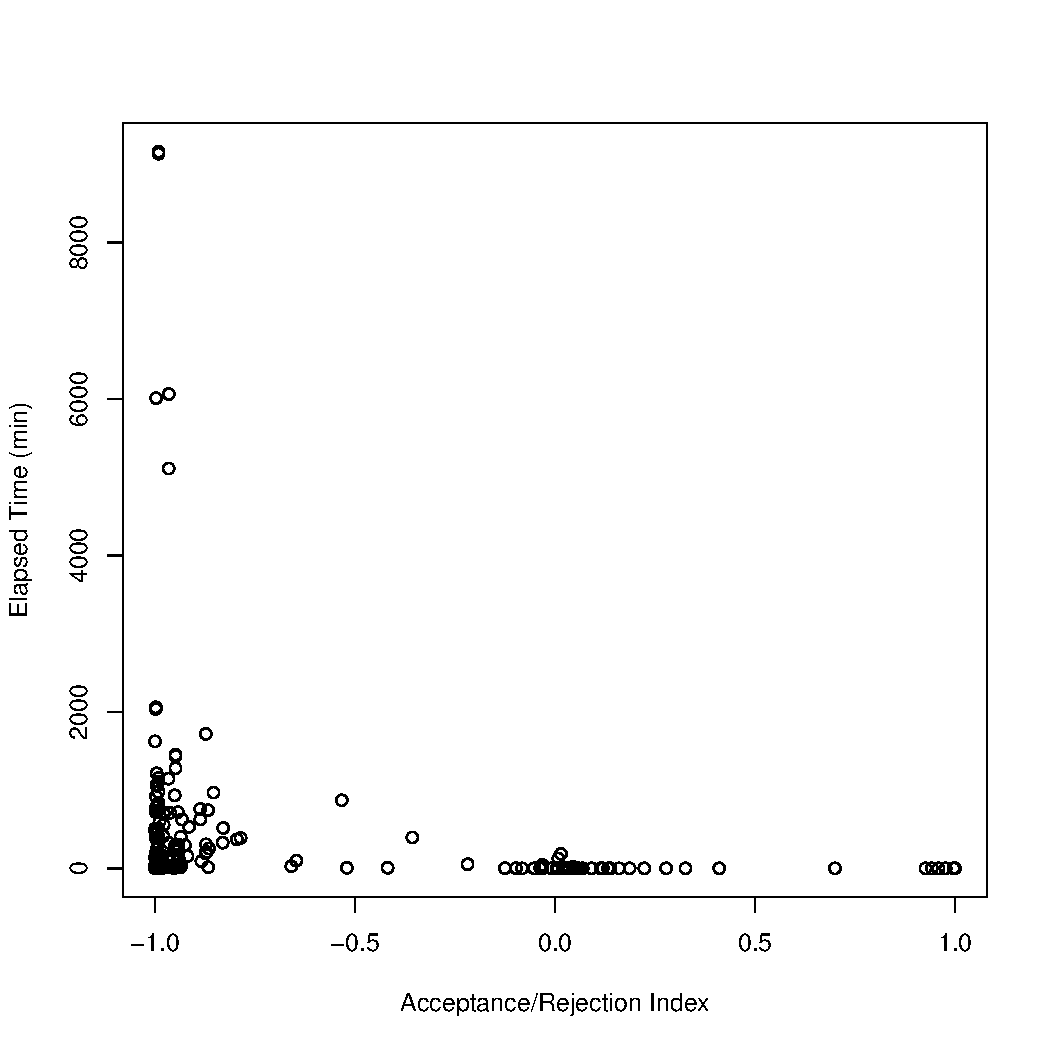
\includegraphics[height=2.25in]{time-ARI} \\
    (a) & (b)
  \end{tabular}
\end{center}
\caption{A histogram showing the distribution of test time of systematically generated
  \textsf{SubClassOf} axioms (a), and a plot of the time taken
  for testing as a function of ARI.}
\label{fig:systematic-time}
\end{figure}

By construction, all axioms generated in this experiment have at least one confirmation
and, as a consequence, non-zero possibility (thus $\mathrm{ARI} > -1$).

\begin{figure}[t]
\begin{center}
  \begin{tabular}{cc}
    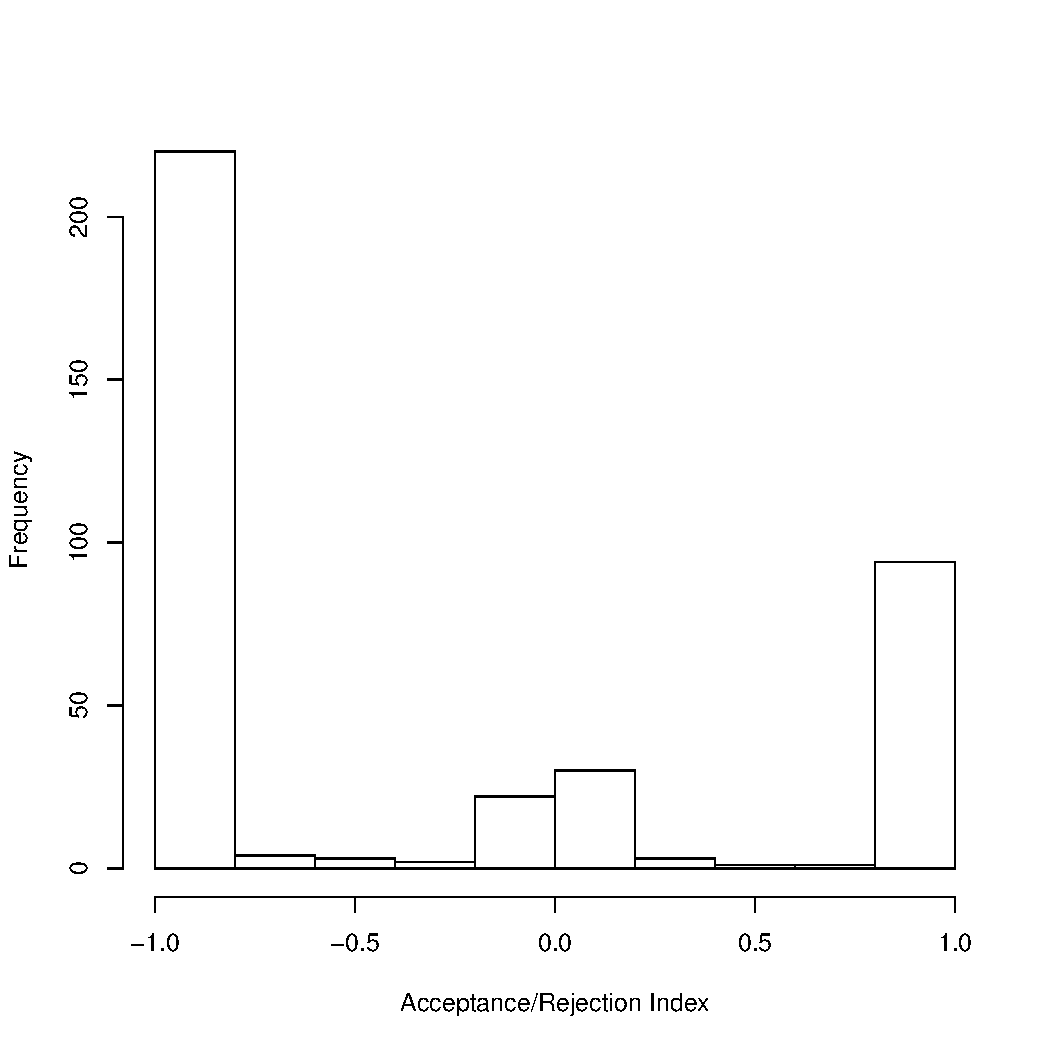
\includegraphics[height=2.25in]{ARI-hist} &
    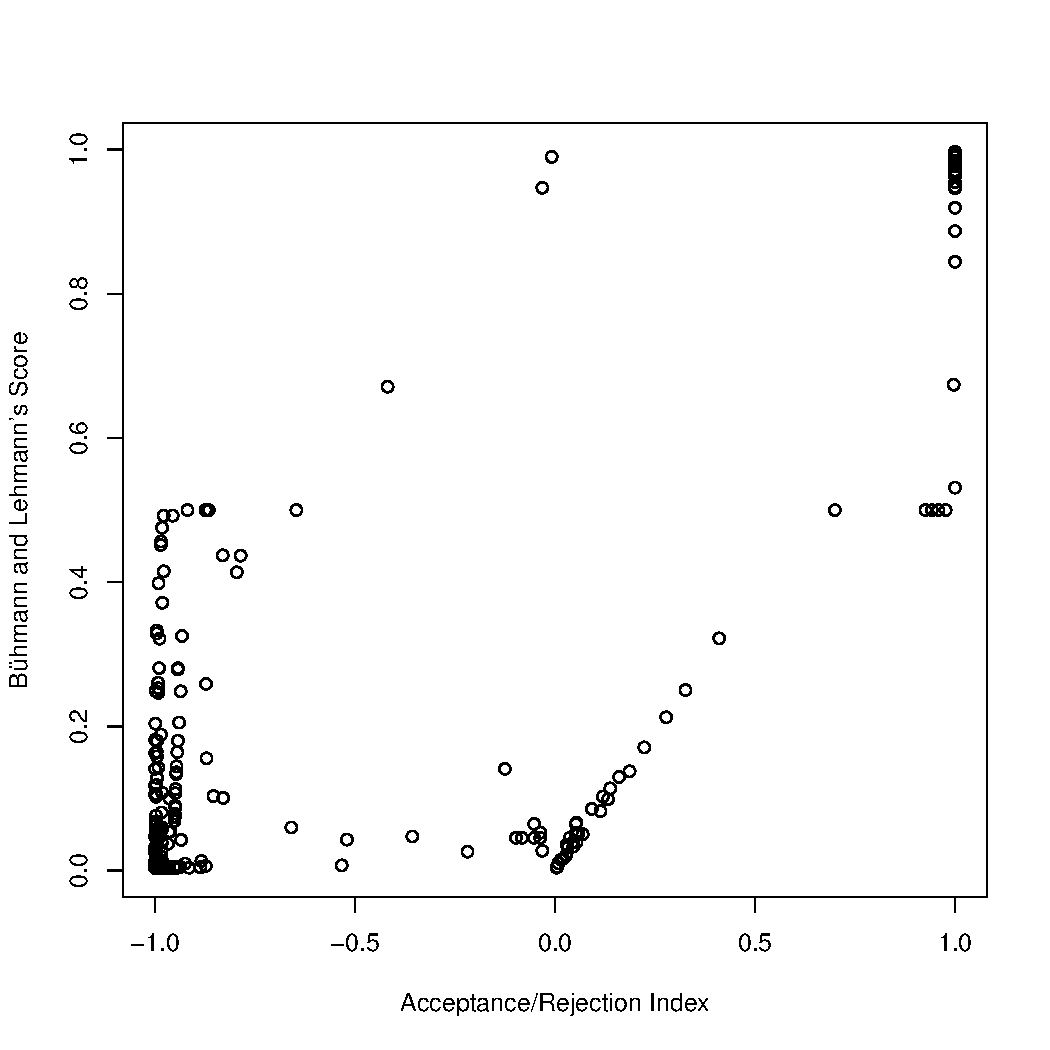
\includegraphics[height=2.25in]{ARI-BLS} \\
    (a) & (b)
  \end{tabular}
\end{center}
\caption{A histogram showing the distribution of the acceptance/rejection index
  of systematically generated \textsf{SubClassOf} axioms (a),
  and the relationship between the acceptance/rejection index and the probability-based
  score used in~\cite{BuehmannLehmann2012} (b).}
\label{fig:ARI}
\end{figure}

The ARI of systematically generated axioms tends to cluster
around the three values $-1$, 0, and 1 (see Figure~\ref{fig:ARI}a).

To assess the discriminatory ability of the proposed scoring heuristics,
we have evaluated these results by sorting the
% UPDATE AS MORE AXIOMS ARE TESTED:
137
tested axioms by their ARI and by manually tagging each of them as either \emph{true} or \emph{false} based on common sense.
Starting from the axioms having an ARI of 1 and proceeding backwards, the first
false axiom encountered was \textsf{SubClassOf(schema:Product gml:\_Feature)},
with an ARI of 0.326187. A positive ARI means no counterexamples were found;
the 2,806 confirmations are all instances of classes \textsf{dbo:Aircraft} and
\textsf{dbo:Ship} having, strangely enough, geographical coordinates.
Three false axioms of the form \textsf{SubclassOf($C$ skos:Concept)},\footnote{Their
confirmations are obvious mistakes: no individual should be a \textsf{skos:Concept}.
This issue appears now to have been fixed in the live version of DBpedia.}
are next, with ARI values comprised between 0.13256 and 0.27782.
The axiom \textsf{SubClassOf(dbo:Award gml:\_Feature)} is also false, with
an ARI of 0.058483. Its four confirmations are \textsf{:St.\_Louis\_Walk\_of\_Fame},
\textsf{:Nobel\_Peace\_Prize}, \textsf{:Candide\_Preis}, and \textsf{:Atrium\_Award},
also having geographical coordinates. The next two axioms with positive ARI are
false too (\textsf{SubClassOf(sche\-ma:Museum foaf:Person)}, with an ARI of 0.031754
and two confirmations, namely \textsf{:Lily\_Safra} and \textsf{Jan\_Hulsker},
and \textsf{SubClassOf(dbo:Award foaf:Person)}, with an ARI of 0.0292509 and
\textsf{:W.\_Wallace\_Mc\-Dowell\_Award} as its only confirmation).
All axioms with a negative ARI were tagged as false, with the exception of
\textsf{SubClassOf(schema:Museum dbo:Building)}, with an ARI of $-0.031754$,
3,957 confirmations and the two exceptions \textsf{:US\_90} and
\textsf{:Saint\_Peter's\_Basilica}.

Selecting an obvious $\mathrm{ARI}(\phi)>0$ as the criterion for acceptance of candidate axiom $\phi$
would thus have yielded 7 false positives and 1 false negative, whereas setting
the acceptance threshold optimally somewhere above 0.33 would have yielded
just one false negative (i.e.\ a
% UPDATE AS MORE AXIOMS ARE TESTED:
99.27\%
accuracy).
However, it appears that the misclassification of the above axioms is to blame
on mistakes in DBpedia. This highlights the potential for the proposed heuristics
as a tool for RDF data validation: confirmations and counterexamples of axioms
with ARI around zero is where the search for bugs should focus.

It is interesting to compare these results with those one would obtain by using
a probability-based score. Figure~\ref{fig:ARI}b provides a comparison by plotting
each axiom according to its ARI (X-axis) and its score computed as in~\cite{BuehmannLehmann2012}
(Y-axis). First of all it is clear that both scores tend to agree in the extremes,
with some notable exceptions, but behave quite differently in all other cases.
The single axiom with probabilistic score close to 1 and slightly negative ARI
is \textsf{SubClassOf(schema:Museum dbo:Building)}; in this specific case, the
probabilistic score appears to fare better than the ARI. However, there are several
true axioms with positive ARI, which get probabilistic scores below the 0.7 threshold
used by~\cite{BuehmannLehmann2012} and would thus be rejected: here it is the ARI
who gives the correct classification.
Finally, most false axiom candidates get an ARI close to $-1$, whilst their
probabilistic scores are almost evenly distributed between 0 and 0.5. We might
say that, besides being more accurate, ARI gives clearer indications than
the probabilistic score.

For the second, more validation-oriented experiment, we extracted an exhaustive
list of \textsf{SubClassOf} axioms in the DBpedia ontology, in functional syntax, with the query
\begin{verbatim}
SELECT DISTINCT concat("SubClassOf(<",str(?x),"> <",str(?y),">)")
WHERE { ?x a owl:Class . ?x rdfs:subClassOf ?y }\end{verbatim}
thus obtaining 541 axioms. Testing them took ``only'' 1 h 23 min 31 s, due to
the fact that most of these axioms have a positive ARI and can thus be tested
relatively rapidly.

%Figure~\ref{fig:time} shows the distribution of the time testing each axiom took,
%as well as a plot showing that such time tends to be proportional to the axiom's
%reference cardinality, i.e., the number of its potential falsifiers.
%Testing time appears to follow a power law: most axioms take less than a minute
%to be tested, but a few of them may even take hours.
%%cath essayer d'expliquer pourquoi et donc de couper quand le temps dépasse une limite

%\begin{figure}[t]
%\begin{center}
%  \begin{tabular}{cc}
%    \includegraphics[height=2.25in]{time-hist} &
%    \includegraphics[height=2.25in]{time-refc} \\
%    (a) & (b)
%  \end{tabular}
%\end{center}
%\caption{A histogram showing the distribution of the elapsed time for testing
%  DBpedia ontology \textsf{SubClassOf} axioms (a), and a plot of the time taken
%  for testing each individual axiom as a function of their reference cardinality.}
%\label{fig:time}
%\end{figure}

A large number of these axioms (143) turned out to have $u_\phi = 0$ (empty support)
thus their ARI is 0. For 28 axioms, a negative ARI signals the presence of
erroneous facts: for example,
\textsf{SubClassOf(dbo:LaunchPad dbo:Infrastructure)} is falsified by \textsf{:USA},
\textsf{SubClassOf(dbo:Brain dbo:AnatomicalStructure)} by \textsf{:Brain} [\emph{sic}],
\textsf{SubClassOf(dbo:Train dbo:MeanOfTransportation)} by
  \textsf{:New\_Jersey\_Transit\_rail\_op\-er\-ations} and \textsf{:ALWEG},
\textsf{SubClassOf(dbo:ProgrammingLanguage dbo:Software)} by \textsf{:Ajax},
\textsf{SubClassOf(dbo:PoliticalParty dbo:Organisation)} by
  \textsf{:Guelphs\_and\_Ghibellines}, \textsf{:New\_People's\_Army},
  \textsf{:-},\footnote{That is \texttt{<}\url{http://dbpedia.org/resource/-}\texttt{>}.
  This IRI is dereferenced to the ``hyphen-minus'' resource.} and \textsf{:Syrian}, etc.

\section{Conclusion}
\label{conclusion}

%The paper should be no longer than 16 pages.
We have proposed a candidate axiom scoring heuristics based on possibility theory
and inspired by Karl Popper's approach to epistemology.
%cath Peut-être commencer par insister sur le fait qu'on veut faire de l'induction d'axiomes à partir des données que c'est dans le but de faire de l'induction d'axiomes à partir des données
%cath et reprendre les terme de la research question pour moontrer qu'on y a bien répondu
%cath une autre contribution est aussi le framework proprement dit for candidate axiom testing
The proposed heuristics is to be used for automatic axiom induction from RDF data
and, ultimately, to provide a solid basis for ontology learning.
By our proposal, we have shown that the falsifiability criterion can indeed be applied
to the task of testing candidate axioms for ontology learning.

In addition, we have developed a framework based on the proposed heuristics,
which uses the model-theoretic semantics of OWL~2 and SPARQL queries to test
candidate axioms.

The results of experimental evaluation on the DBpedia dataset clearly indicate
that the proposed heuristics is suitable for tasks such axiom
induction and ontology learning and, furthermore, may be beneficial as a tool
for ontology and knowledge-base validation.

%cath je trouve le paragraphe qui suit un peu rude comme fin. Pourrait venir plus tôt?
One may object that, being based on possibility theory, our scoring heuristics
is less objective than a probability-based scoring method. However, we have argued
in Section~\ref{probability} that scoring heuristics based on probability are doomed
to be arbitrary and subjective or, in other words, \emph{qualitative}
and, therefore, hardly more rigorous or objective than the proposed approach.
The experimental results corroborate this claim.

%cath on pourrait classiquement terminer par des perspectives:
%continuer l'expérience, en mettant un time out
%traiter de nouveaux axiomes
Future work includes extending the experimental evaluation to more general sets
of candidate axioms and enlarging the test base by including additional RDF datasets
from the LOD.
We also plan on improving the implementation of the framework by setting a time-out
on query evaluation to reduce the computational overhead of axiom testing.

\bibliographystyle{tetta-lncs}
\bibliography{../RDFMining}
\end{document}

